\section{Einleitung}
%\lbrack Zitat (optional)\rbrack :
%\begin{quote}
%\glqq Was ist die Absicht eines wissenschaftlichen Buches? Es stellt Gedanken 
%dar und will den Leser von ihrer Gültigkeit überzeugen. Darüber hinaus will 
%der Leser auch wissen: woher kommen diese Gedanken und wohin führen sie? Mit 
%welchen Richtungen auf anderen Gebieten hängen sie zusammen?\grqq
%\pcite{}{XVII}{carnap1974}
%\end{quote}
Die Cloud ist im Mainstream angekommen. \pcite{}{}{thoughtsOnCloud} Wie in 
Abbildung ~\ref{umsatz_cloud_computing_weltweit} darsgestellt, wuchs der 
weltweite Umsatz mit Cloud-Computing von 58,6 Milliarden US-Dollar im 
Jahr 2009 auf geschätzte 203,9 Milliarden US-Dollar im Jahr 2016, was einem 
durchschnittlichen jährlichen Wachstum von 16,87\%\footnote{CAGR(2009,2016) = 
16,87\%} entspricht. \pcite{}{}{CloudUmsatzWeltweit} \\
Auch deutsche Unternehmen drängen zunehmend in die Cloud. Das 
Marktforschungsunternehmen PAC schätzt, dass der 
deutsche Cloud-Markt im Jahr 2016 eine Größe von 12,5 Milliarden Euro hatte und 
mit durchschnittlich jährlich 20,9\%\footnote{CAGR(2016,2020) = 20,9\%} auf 31,4 
Milliarden im Jahr 2020 anwächst. Im deutlichen Gegensatz dazu prognostiziert 
PAC für den Markt der traditionellen IT-Dienstleistungen ein negatives Wachstum 
von  -1,7\%\footnote{CAGR(2015,2019) = -1,7\%}. \pcite{}{}{MarketVision}

\begin{figure}[bh]
\begin{center}
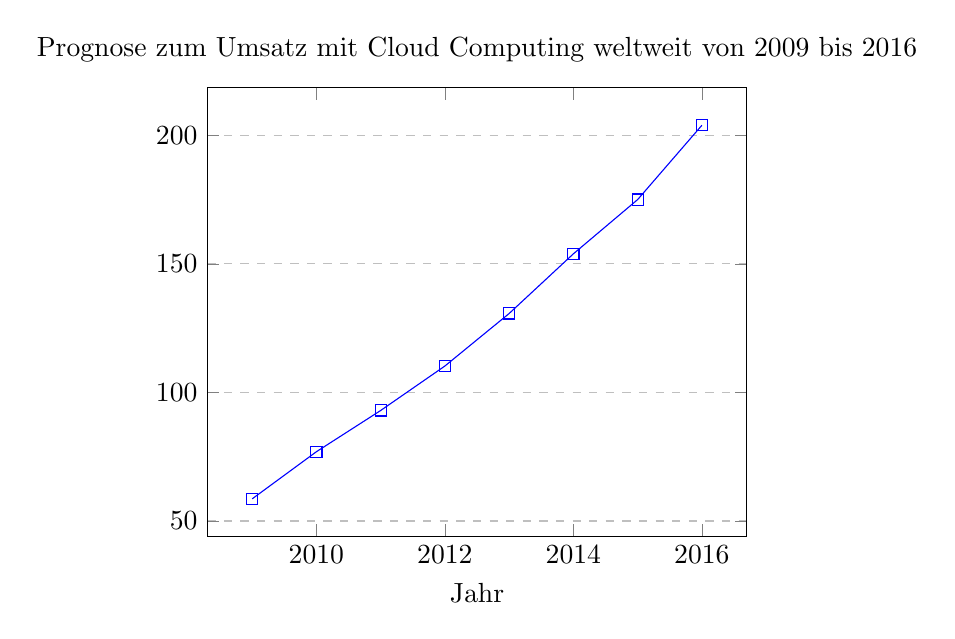
\begin{tikzpicture}
\begin{axis}[
/pgf/number format/.cd,
        use comma,
        1000 sep={},
    title={Prognose zum Umsatz mit Cloud Computing weltweit von 2009 bis 2016},
    xlabel={Jahr},
    %ylabel={Umsatz [Mio. US-Dollar]},
    %xmin=2012, xmax=2016,
    %ymin=0, ymax=8000,
    %xtick={0,20,40,60,80,100},
    %ytick={0,20,40,60,80,100,120},
    legend pos=north west,
    ymajorgrids=true,
    grid style=dashed
]

\addplot[color=blue,mark=square,]
    coordinates {
	(2009,58.6)
	(2010,76.94)
	(2011,92.97)
	(2012,110.27)
	(2013,130.7)
	(2014,153.91)
	(2015,175)
	(2016,203.9)
    };
    %{Cloud Umsatz weltweit}
    
%\addplot[color=green,mark=square,]
%    coordinates {
%    
%(2009,0)(2010,0)(2011,0)(2012,2.267)(2013,3.050)(2014,4.071)(2015,5.374)(2016
% ,6.667)
%    };
    %\legend{Salesforce}
 
\end{axis}
\end{tikzpicture} 
\caption{Prognose zum Umsatz mit Cloud Computing weltweit von 2009 bis 2015 mit 
geschätztem Wert für 2016 entnommen aus \cite{CloudUmsatzWeltweit} }
\label{umsatz_cloud_computing_weltweit}

\end{center}
\end{figure}


Gerade Softwarehersteller aus diesem traditionellen Bereich der 
IT-Dienstleistungen sehen sich unter Druck gesetzt, ihre 
Unternehmungen von diesem schrumpfenden Markt weg, in den stark wachsenden 
Cloud-Markt zu verlagern. Dabei ist es intuitiv vernünftig, vorhandene 
Kernkompetenzen durch Migrationen bestehender Produkte zu nutzen, um 
Wettbewerbsvorteile auf dem neuen Markt zu erlangen. \\
Doch nicht nur die Umsatzentwicklung des Marktes setzt die Softwarehersteller 
unter Druck: Ihre Kunden haben sich an Anwendungen in der Cloud gewöhnt und
erwarten sich - von ihr - eine günstigere, schnellere, einfachere, flexiblere 
und effizientere IT im Allgemeinen. \pcite{}{}{economics_of_the_cloud}
\begin{comment}
Günstiger, weil bei der Beschaffung, der Wartung und dem 
Betrieb des Rechenzentrums Skalenerträge erzielt werden können. Schneller, weil 
Cloud-Anbieter Leistungsreserven in einem Umfang bilden können und müssen, wie 
es für einzelne Firmen in ihren IT-Landschaften kaum möglich ist. Einfacher, 
weil Cloud-Dienste in der Regel auch mit Mobilgeräten gut bedienbar sind. 
Flexibler, weil sich Leistungen unkompliziert über das Internet buchen lassen 
und automatisch skalieren. Effizienter, weil nur der Umfang bezahlt wird, 
der auch genutzt wird. \pcite{}{}{economics_of_the_cloud} \\ 
\end{comment}

Diese bei den Nutzern geweckten Erwartungen sorgen bei den Softwareherstellern 
für zusätzlichen Migrationsdruck, sie setzen aber auch einen neuen, höheren 
Maßstab für Software im Allgemeinen.

Entschließt sich ein Softwarehersteller dazu, seine Produkte 
als Dienstleistungen in der Cloud anzubieten, ändert sich nicht nur die 
technologische, sondern auch die wirtschaftliche Umgebung erheblich, da ein 
neuer Markt erschlossen wird und bedacht werden muss, wie und wo die 
Cloud-Lösung auf dem Markt zu positionieren ist. Die Position im Wettbewerb hat 
nicht nur für das Vertriebsmodell  Auswirkungen - man 
denke an Fragen der Lizenzierung und Preismodelle - sondern auch den 
Leistungsumfang. Denn je standardisierter eine Software ist, je 
geringer die nötige Anpassbarkeit, desto wahrscheinlicher lassen sich bei einem 
Betrieb in der 
Cloud die genannten Vorteile realisieren. \pcite{}{}{saasBuxmann2008} Dies 
hängt damit zusammen, dass sich bei standardisierter Software Stellschrauben 
vor dem Nutzer verbergen lassen. Im Optimalfall spielen Netzwerktopologie, 
Betriebssystem, Laufzeitumgebung und Datenbanken keine Rolle; der Anwender 
sieht und arbeitet lediglich mit der Software. In diesem Fall spricht man von 
"`Software as a Service"' (SaaS). \pcite{}{11}{economics_of_the_cloud}


\begin{comment}
Als SaaS-Vertriebsplattform soll in dieser Arbeit schwerpunktmäßig Salesforce 
betrachtet werden, das mit "`AppExchange"' einen Marktplatz zur Verfügung 
stellt, auf dem Hersteller ihre auf der Salesforceplattform laufenden 
Anwendungen anbieten können. Die Konzentration auf Salesforce als Zielplattform 
war zum einen durch das Unternehmen gegeben, mit dem in freundlicher 
Kooperation diese Thesis entstanden ist.

\begin{figure}[bh]
\begin{center}
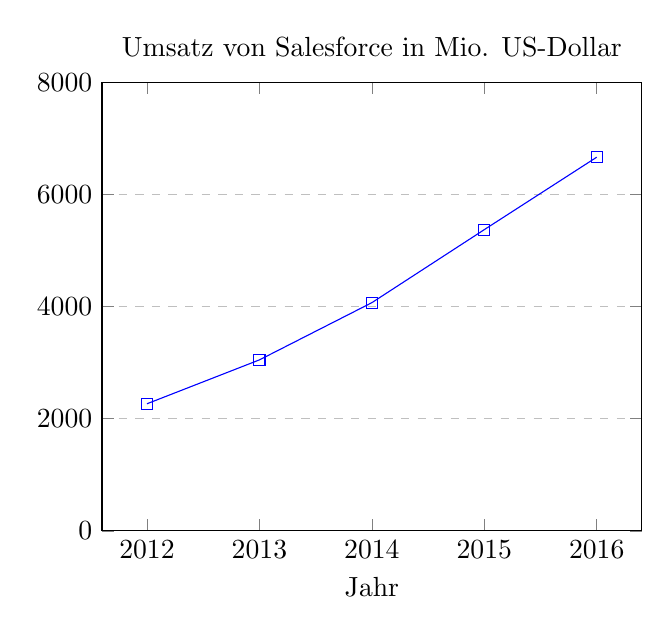
\begin{tikzpicture}
\begin{axis}[
/pgf/number format/.cd,
        use comma,
        1000 sep={},
    title={Umsatz von Salesforce in Mio. US-Dollar},
    xlabel={Jahr},
    %ylabel={Umsatz [Mio. US-Dollar]},
    %xmin=0, xmax=100,
    ymin=0, ymax=8000,
    %xtick={0,20,40,60,80,100},
    %ytick={0,20,40,60,80,100,120},
    legend pos=north west,
    ymajorgrids=true,
    grid style=dashed
]

\addplot[color=blue,mark=square,]
    coordinates {
    (2012,2267)(2013,3050)(2014,4071)(2015,5374)(2016,6667)
    };
    %\legend{Salesforce}
 
\end{axis}
\end{tikzpicture}
\caption{Umsatzzahlen entnommen aus \cite[43]{salesforceannualreport} }
\label{UmsatzzahlenSalesforce}
\end{center}
\end{figure}
Zum anderen aber gehört Salesforce neben Microsoft 
und Google zu den größten SaaS-Anbietern
\pcite{}{247}{softwareindustrie2015} und konnte zwischen 2012 und 2016 
den Umsatz mit durchschnittlich 31\% von 2,267 Milliarden US-Dollar auf 
6,667 Milliarden US-Dollar rasant steigern (Vgl. Abbildung 
~\ref{UmsatzzahlenSalesforce}). Daher dürfte es als Zielplattform für 
viele Unternehmen eine Option sein.
\end{comment}

In der Literatur finden sich zahlreiche Vorgehensmodelle, die 
versuchen, die Migration eines Altsystems beziehungsweise einer Altsoftware 
in die Cloud im 
weitesten Sinne zu strukturieren. In einigen, wie in dem von 
\citeflow{framework_for_architecture-driven_migration} entwickelten Modell wird 
ein technischer Schwerpunkt gesetzt; wirtschaftliche Aspekte bleiben weitgehend 
unberücksichtigt. Andere fokussieren sich lediglich auf den Kosten-Faktor 
(\citeflow{fivephases}). Umfassendere Modelle 
(\citeflow{migrating_applications_to_public_cloud_services}) betonen die 
markt-strategischen Folgen einer Cloud-Migration für Unternehmen. 

Zielgruppe der Modelle sind in der Regel Unternehmen, die Teile ihrer 
IT-Landschaft in die Cloud migrieren wollen. Dies kann zum Beispiel ein 
Unternehmen sein, das 
seine Lagerhaltung in die Cloud verlagern will. Eine in 
dieser Arbeit durchgeführte Literaturrecherche ergab, 
dass Softwarehersteller als Zielgruppe bisher vernachlässigt wurden. Der 
Unterschied zwischen den beiden Gruppen ist gravierend: Während im oben 
genannten Beispiel die 
Lagerhaltung in Form einer Software lediglich das Kerngeschäft unterstützt, 
besteht für den Softwarehersteller das Kerngeschäft in der zu migrierenden 
Software. Für den Erfolg im Wettbewerb ist eine strategische 
Neuausrichtung 
unabdingbar, unterscheidet sich in ihrer Tragweite und ihrem Umfang jedoch 
erheblich von den strategischen Überlegungen, die ein Unternehmen einer anderen 
Branche bei der Cloud Migration treffen muss. 

Um diese Forschungslücke zu schließen, soll ein Modell entwickelt werden, das 
Softwarehersteller bei der Migration in die Cloud unterstützen soll. Grundlage 
ist eine Literaturrecherche, die die folgenden Fragen klären soll:
\begin{enumerate}
	\item Welche Merkmale (Chancen und Risiken) der Cloud sind bei der 
Migration zu berücksichtigen?
	\item Wie beeinflussen die gefundenen Merkmale die strategische 
Ausrichtung und das Geschäftsmodell eines Softwareherstellers?
	\item Wie beeinflussen die gefundenen Merkmale den Migrationsprozess 
eines Softwareherstellers?
\end{enumerate}

Bevor diese Fragen in Kapitel~\ref{cha:entwicklung_vorgehensmodell}  
beantwortet werden und in der Entwicklung eines Vorgehensmodells resultieren, 
wird in Kapitel ~\ref{cha:grundlagen} auf grundlegende Fragen eingegangen: 
Welche Vorteile verspricht die Cloud und wie lassen sie sich erzielen? Auf 
welche Weise unterschiedet sich eine Cloud-Migration von herkömmlichen 
Migrationen in der IT? Was wird in dieser Arbeit unter einem Softwarehersteller 
verstanden und welche Annahmen werden getroffen? Wie wirken sich dessen 
Charakteristika auf die Migration aus?
Um Erfahrungen aus der Praxis in das 
Modell einzubeziehen, wurde das entwickelte Modell in Zusammenarbeit mit einem 
Beratungsunternehmen auf ein reales Projekt angewendet; Unternehmen und Projekt 
werden ebenfalls in diesem Kapitel vorgestellt.
Das Grundlagenkapitel schließt mit der Vorstellung des Fünf-Phasen-Modells, das 
als Basis und Orientierung für das in dieser Arbeit entwickelte Modell dient.

Kapitel~\ref{cha:method} beschreibt die Literaturrecherche mit der die 
Forschungsfragen beantwortet wurden. Um praktische Erfahrungen einfließen zu 
lassen wurden Gespräche mit Mitarbeitern geführt, deren Ablauf ebenfalls in 
diesem Kapitel geschildert werden.

In Kapitel~\ref{cha:result} wird das Vorgehensmodell beispielhaft auf das zu 
migrierende Projekt aus der Praxis angewendet; es werden Möglichkeiten 
dargestellt, um Chancen der Cloud zu realisieren und Risiken zu meiden -- auch 
in Bezug auf das Geschäftsmodell.

In Kapitel~\ref{cha:diskussion} werden die Unterschiede zwischen 
vorgeschlagenem und tatsächlichem Vorgehen herausgearbeitet und diskutiert.

Die Ergebnisse dieser Diskussion werden anschließend in Kapitel~\ref{cha:fazit} 
zusammengefasst, offene Fragestellungen, Herausforderungen und Forschungsfragen 
formuliert.
\begin{comment}


Lösungen 
haben ganz allgemein zwei Vorteile für Unternehmen, die am für Salesforce 
typischen Beispiel einer Kundenverwaltung schildern möchte. Möchte ein 
Unternehmen Informationen zu seinen Kunden zentral speichern, muss es bei einer 
Cloudlösung keinen Server installieren und warten. Es kann also Kosten für 
Hardware sowie mindestens noch Personalkosten bei der Administration einsparen. 
Der erste Vorteil entsteht also durch Kosteneinsparungen auf Serverseite des 
Unternehmens. Cloudbasierte Software lässt sich regelmäßig mit einem Browser 
bedienen, der auf allen mobilen und internetfähigen Geräten wie auf 
herkömmlichen Computern verfügbar sein dürfte. Im Beispiel muss der Anwender, 
der Zugriff auf die Kundendaten nehmen will, keine Software installieren und 
ist an kein Gerät gebunden.\\
Die Idee hinter dem Migrationsprojekt ist die Verbindung der Expertise beider 
Unternehmen: Die Nutzung des aufgebauten Know-Hows auf einer neuen, 
zukunftsfähigen Plattform. \\
Dabei stellen sich die folgenden Fragen:
\begin{itemize}
	\item Welche Strategie sollte künftig mit dem bestehenden Produkt 
verfolgt werden?
	\item In welchem Umfang soll die Cloud Software durch 
	\begin{itemize}
		\item den Anbieter
		\item den Kunden
	\end{itemize}
	anpassbar sein?
	\item Wie lassen sich idealerweise die Anforderungen ermitteln?
	\item Welche Funktionen sollen übernommen werden?
	\item Wie lässt sich ein bestehendes Produkt an die neuen Möglichkeiten 
der Cloud anpassen?
\end{itemize}

Im folgenden gebe ich einen Überblick über Methoden des 
Requirements-Engineering.
\end{comment}
